\documentclass[a4]{scrartcl}

\usepackage[ngerman]{babel}
\usepackage[utf8]{inputenc}
\usepackage{mathtools}
\usepackage{amsmath}
\usepackage{adjustbox}
\usepackage{amssymb}
\usepackage{geometry}
\usepackage{scrpage2}
\pagestyle{scrheadings}
\usepackage[bottom]{footmisc}
\usepackage{footnote}
\makesavenoteenv{tabular}
\makesavenoteenv{table}
\clearscrheadfoot

\setlength{\parindent}{0em}

\geometry{
  paper=a4paper, % Change to letterpaper for US letter
  top=2cm, % Top margin
  bottom=1.5cm, % Bottom margin
  left=2cm, % Left margin
  right=3cm, % Right margin
  %showframe, % Uncomment to show how the type block is set on the page
}

\ohead{\\
Pina Kolling}


\begin{document}

\subsection*{Vorlesung 6}

\textbf{Digitale Technologien ermöglichen innovative Geschäftsideen} \\
Beispiel: Musik
\\ \\
\adjustbox{max width=\textwidth}{%

\begin{tabular}{c | c c c}

Produkt & CDs & MP$3$-Download & Streaming \\
Vertrieb & Einzelhandel & Download Plattform (Digitales Gut) & Streaming Plattform (Digitales Gut) \\
Kunde & zeitlich unbegrenzte Nutzung, & zeitlich unbegrenzte Nutzung & Nutzung durch Abonnement \\
 & Verschleiß  & & \\

\end{tabular}}

\vspace*{2em}

\textbf{Digitales Gut} 
\begin{itemize}
\item liegen in immaterieller Form vor
\item vollständig als digitale Repräsentation in Binärform gespeichert
\item können ohne Bindung an Trägermedium entwickelt, vertrieben oder angewendet werden (bsp. übers Internet)
\end{itemize}

\textbf{Digitalisierungsgrade von Gütern}

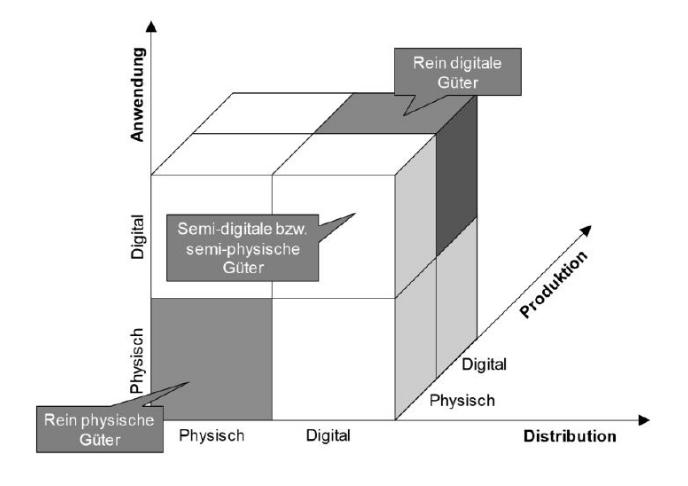
\includegraphics[scale=0.35]{wuerfel.png}

\vspace*{1em}

\textbf{Eigenschaften digitaler Güter} 

\begin{itemize}
\item Wahrnehmungsunterschiede \\
Digitale Güter können nur über zwei Sinne (Sehen und Hören) wahrgenommen werden.
\item Skaleneffekte \\
Keine Kostenvorteile entstehen bei durch sinkende Kosten pro hergestelltem Produkt.
\item Kopierbarkeit/Verteilbarkeit \\
Digitale Güter werden bei Weitergabe vermehrt, nicht aufgeteilt.
\item Veränderbarkeit/Editierbarkeit/Reprogrammierbarkeit \\
Digitale Güter können ohne großen Aufwand in Produktvarianten überführt und angeboten werden.
\item Abnutzbarkeit \\
Digitale Güter unterliegen keinerlei Abnutzung; die Unterscheidung zwischen neuem und altem Gut entfällt.
\end{itemize}

\newpage

\textbf{Physische vs. digitale Güter}
\\
\\
\adjustbox{max width=\textwidth}{%

\begin{tabular}{c c}
Physische Güter & Digitale Güter \\
\hline
Hohe Vervielfältigungskosten & Niedrige Vervielfältigungskosten \\
Angleichung der Grenzkosten\footnotemark \ an die Durchschnittskosten & Grenzkosten der (Re-)Produktion nahe Null \\
Wertverlust durch Gebrauch & Kein Wertverlust durch Gebrauch \\
Individueller Besitz & Vielfacher Besitz (möglich) \\
Wertverlust durch Teilung, begrenzte Teilbarkeit & Kein Wertverlust durch Teilung, fast beliebige Teilbarkeit \footnotemark \\
Identifikations- und Schutzmöglichkeiten \footnotemark & Probleme des Datenschutzes und der Datensicherheit \\
Schwierige Verbreitung (Logistik) & Einfache Verbreitung \\
Preis bzw. Wert im Markt ermittelbar & Preis bzw. Wert nur schwer bestimmbar \\

\end{tabular}}
\footnotetext[1]{Wikipedia: Die Grenzkosten sind die Kosten, die durch die Produktion einer zusätzlichen Mengeneinheit eines Produktes oder einer Dienstleistung entstehen.}
\footnotetext[2]{Persönliche Anmerkung: Serverkosten? Wartung von Software ist auch extrem aufwendig.}
\footnotetext[3]{Persönliche Anmerkung: Schon einmal was von Einbrechern oder Diebstahl gehört? Daten schützen und sein Haus schützen sollten schon auf vergleichbarer Ebene stehen.}





\end{document}






